%! Author = sbbfti
%! Date = 10/06/2020


\section{Results}\label{sec:results}

\subsection{Sensible Heat Loss from the Skin}\label{subsec:sensible-heat-loss-from-the-skin}

The sensible heat losses from the skin to the environment are proportional to the difference between the \ac{t-sk} and \ac{t-op}.
Consequently for values of \ac{t-op} higher than \ac{t-sk} the term \ac{c-r} becomes negative, or in other terms the body gains sensible heat from its environment.
Figure~\ref{fig:comparison_models}A shows how the sensible heat losses estimated with the \ac{set} and the Ollie et al. \mycite{Jay2015} as a function of the \ac{t-db}, \ac{rh}, and \ac{v}.

\begin{itemize}
    \item In the SET model the dry heat losses vary as a function of the relative humidity, since relative humidity affects sweat rate and consequently skin temperature.
    \item In the SET model there is a sharp change in the latent heat loss required which is counter intuitive.
    \item sweat rates are similar, with the only difference that SET sets an upper threshold to 500 mL/h.
    \item max latent heat loss is significantly affected by skin wettedness (w). W can technically range from 0 to 1.
    Ollie states that cannot be higher than 0.65 for young adults and 0.5 for younger adults.
    The ASHRAE fundamentals states ``Azer (1982) recommends 0.5 as a practical upper limit for sustained activity for a healthy, acclimatized person."
    The SET model help us with that since we can use it to estimate the maximum value for w, which only varies as function of the air velocity $w_{max} = 0.59 * v^{-0.08}$
    \item I do not really see the benefit of the model proposed by Hosper since: 1) they set the limit of sweating to 440 mL/h; and they limit 2) the amount of water than I person can spray on him self to 116 mL/h. This would not affect the results in the SET model since with the SET model the estimated sweating rate is lower.
    On the other hand it affects the result in the Ollie model since the exponential growth of the sweat rate in their model is more marked.
    Moreover, very dry climates could benefit from using evaporative cooling.
\end{itemize}

Figure~\ref{fig:core_body_tmp}.

\begin{itemize}
    \item The core body temperature is lower for high air speed when temperatures and relative humidity are low.
    Core body temperature can be used to determine when to use fan or not.
\end{itemize}

\begin{figure}
    \centering
    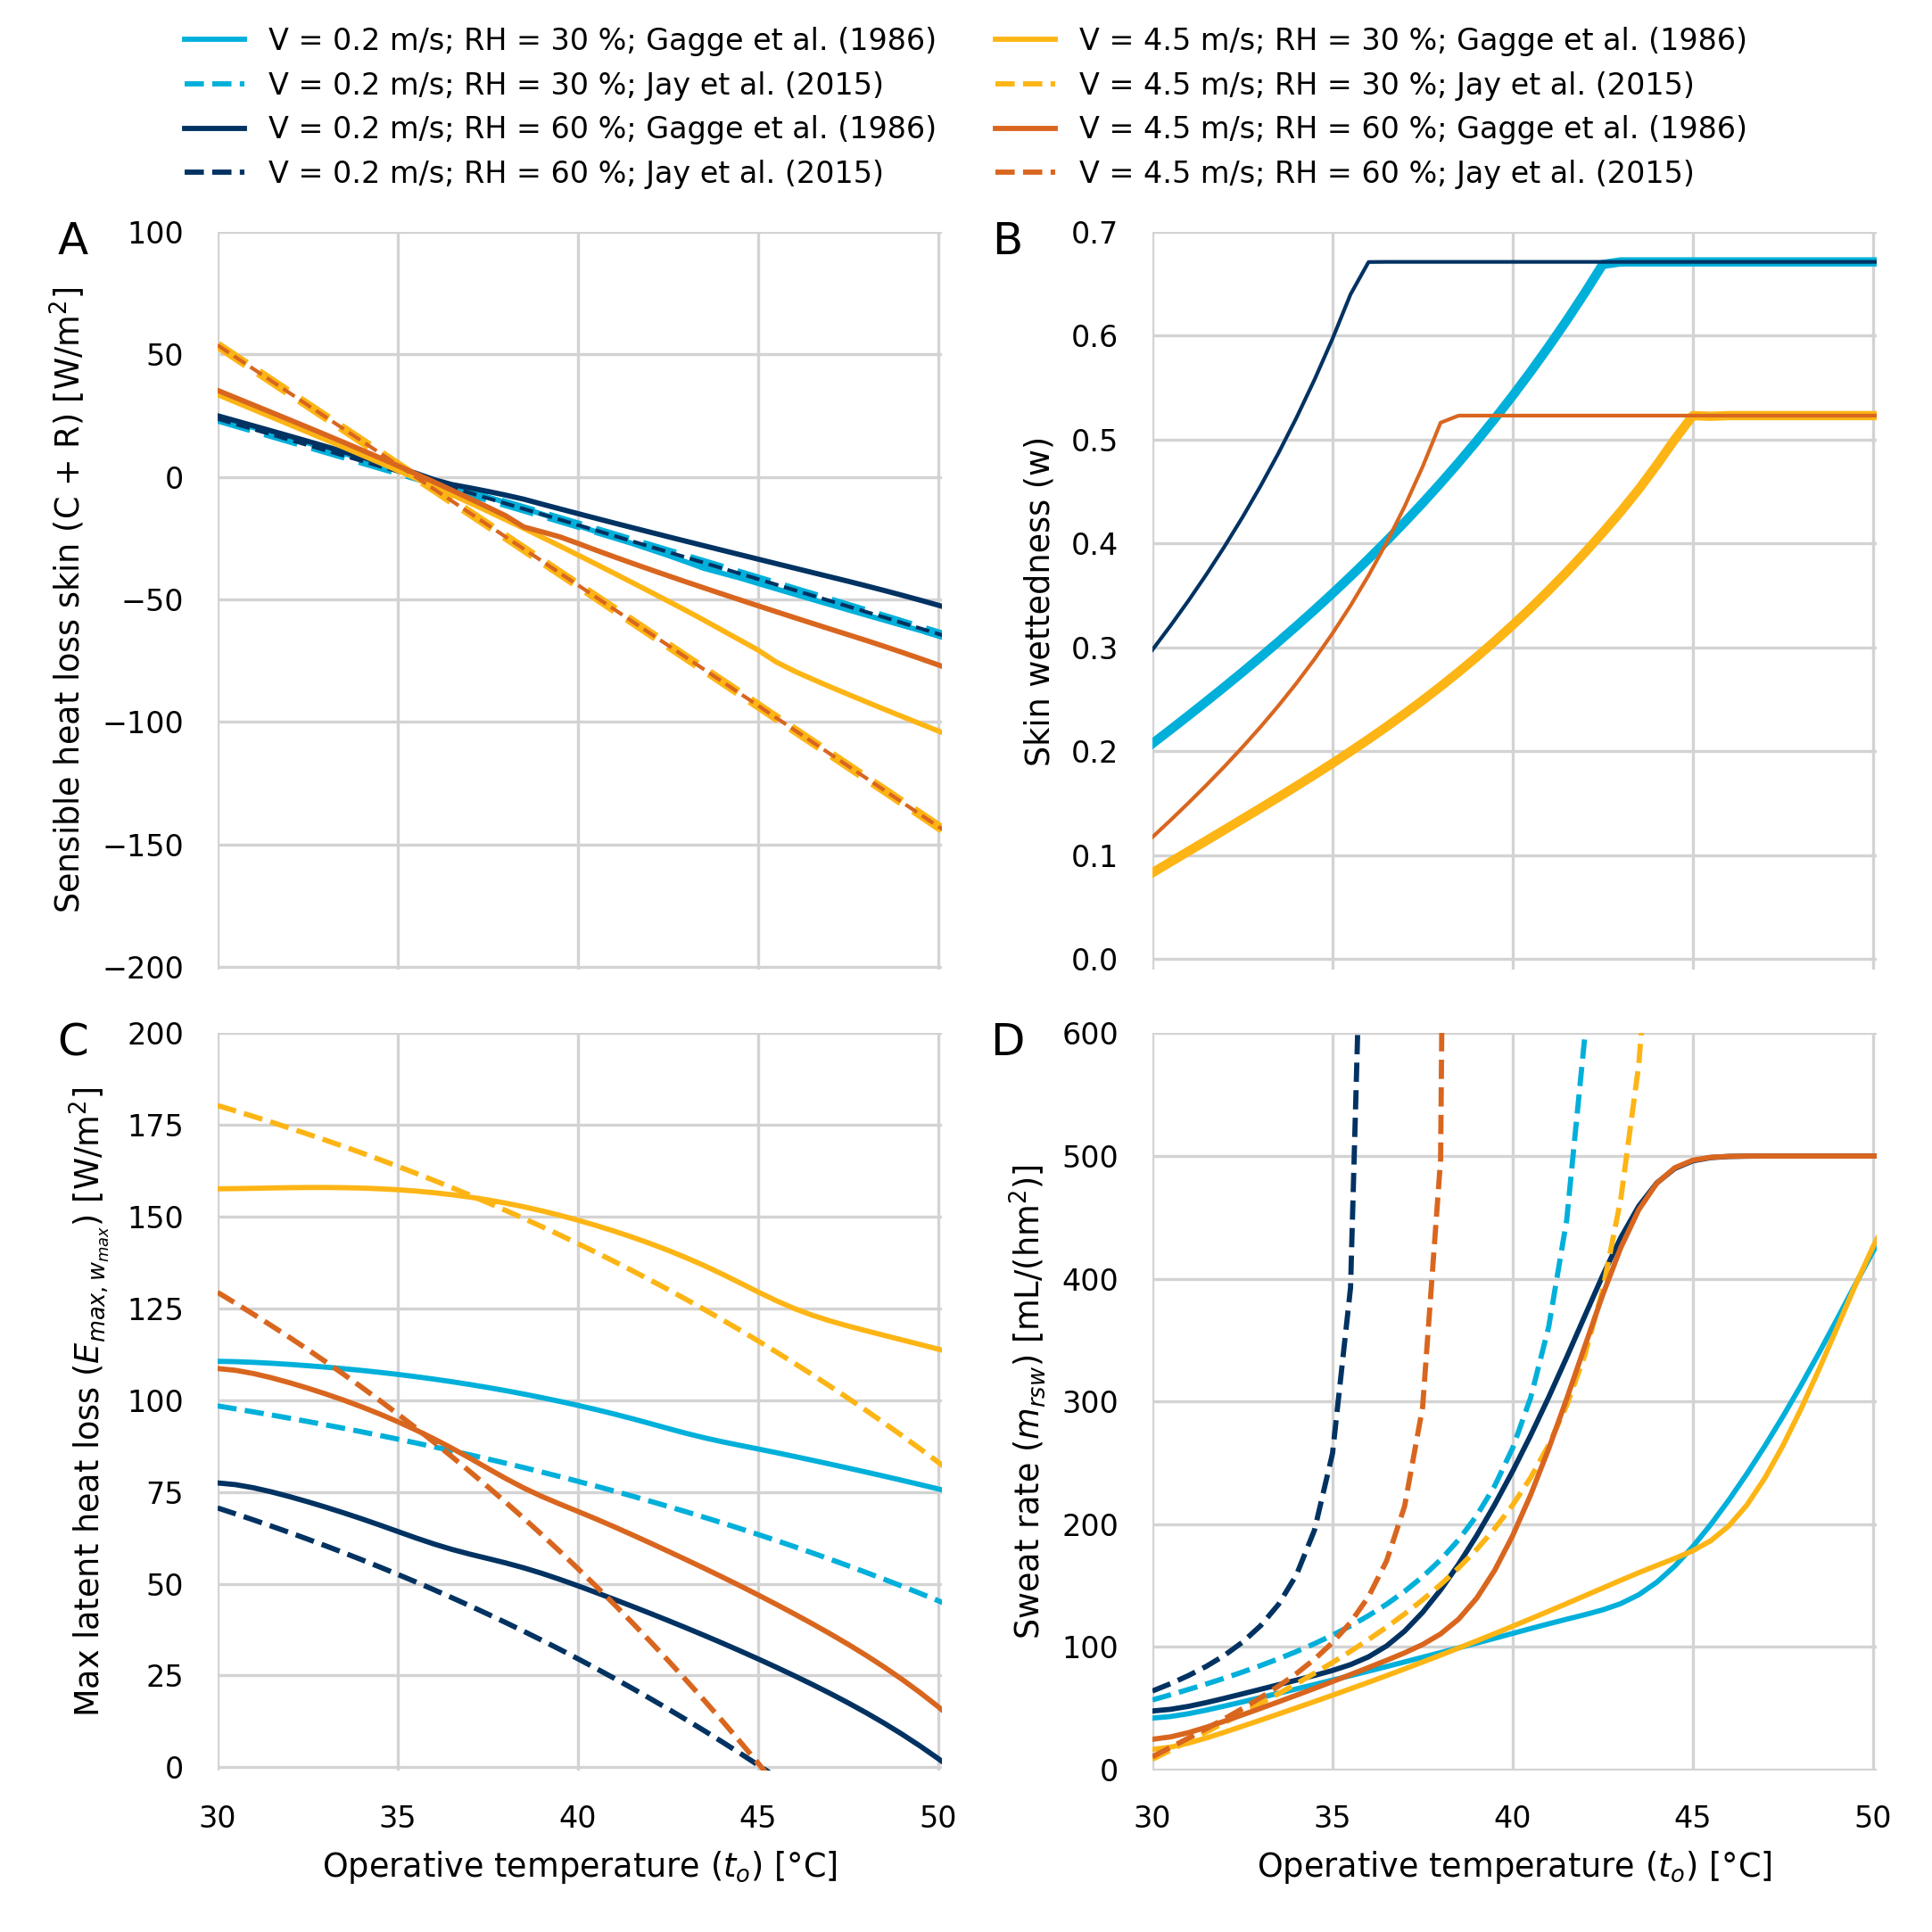
\includegraphics[width=\textwidth]{figures/comparison_models_v2.png}
    \caption{Caption}
    \label{fig:comparison_models}
\end{figure}

\begin{figure}
    \centering
    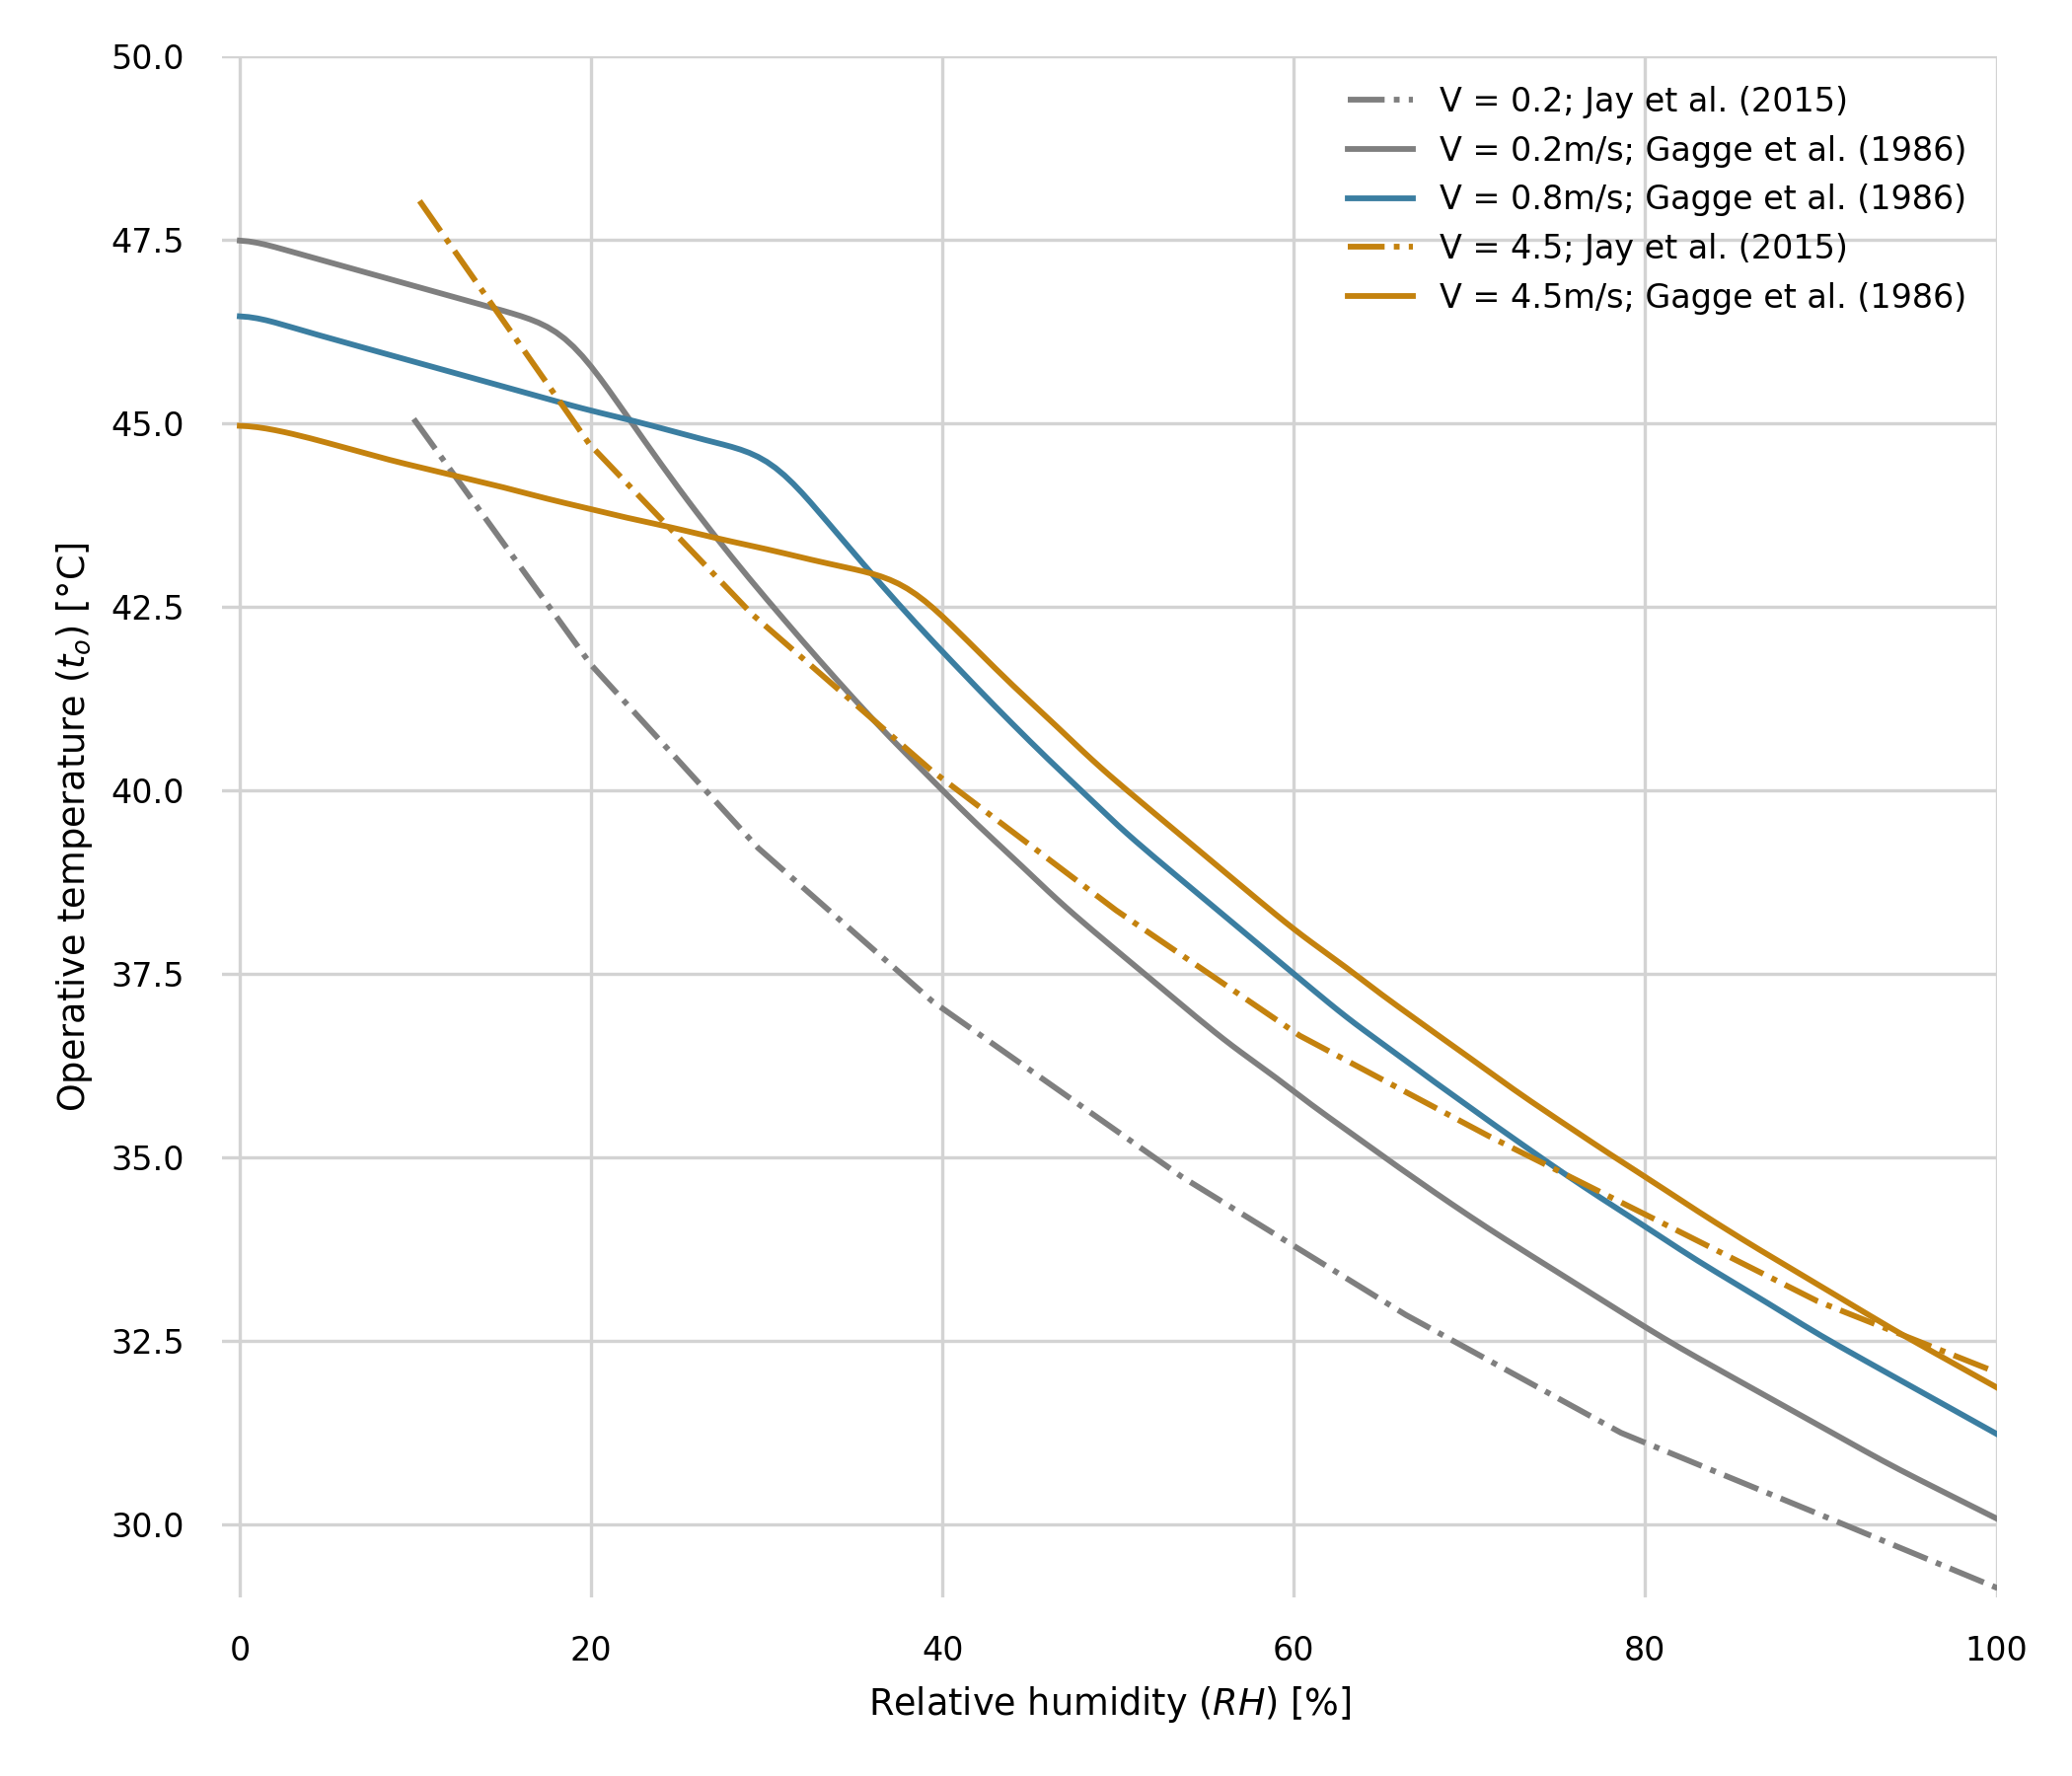
\includegraphics[width=\textwidth]{figures/comparison_air_speed.png}
    \caption{Compares the results between the SET model and Ollie's model.
    Each line demarcates the boundary between acceptable cardiovascular strain (below line) and elevated cardiovascular strain (above the line).
    Above the line the latent heat that needs to be dissipated exceeds the amount of latent heat that the same individual can dissipate. }
    \label{fig:comparison_air_speed}
\end{figure}

\begin{figure}
    \centering
    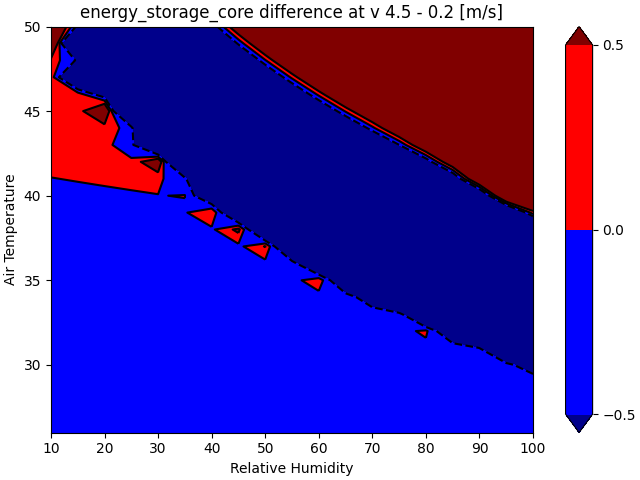
\includegraphics[width=\textwidth]{figures/energy_storage_delta.png}
    \caption{Caption}
    \label{fig:energy_storage_delta}
\end{figure}

\begin{figure}
    \centering
    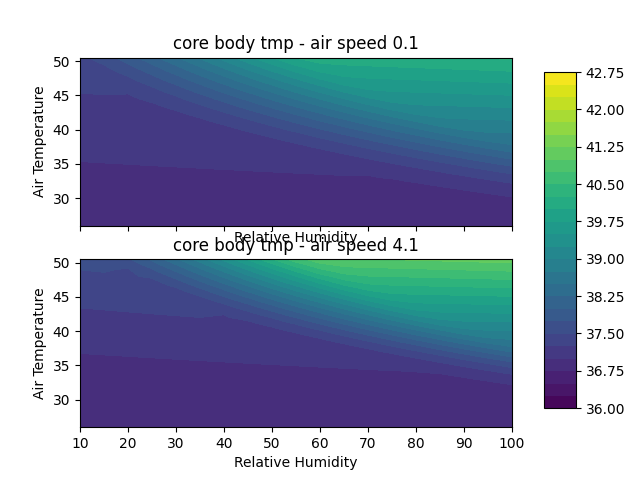
\includegraphics[width=\textwidth]{figures/core_body_tmp.png}
    \caption{Caption}
    \label{fig:core_body_tmp}
\end{figure}


